\documentclass[tikz,border=4pt]{standalone}
\usepackage{pgfplots}\pgfplotsset{compat=1.18}
\begin{document}
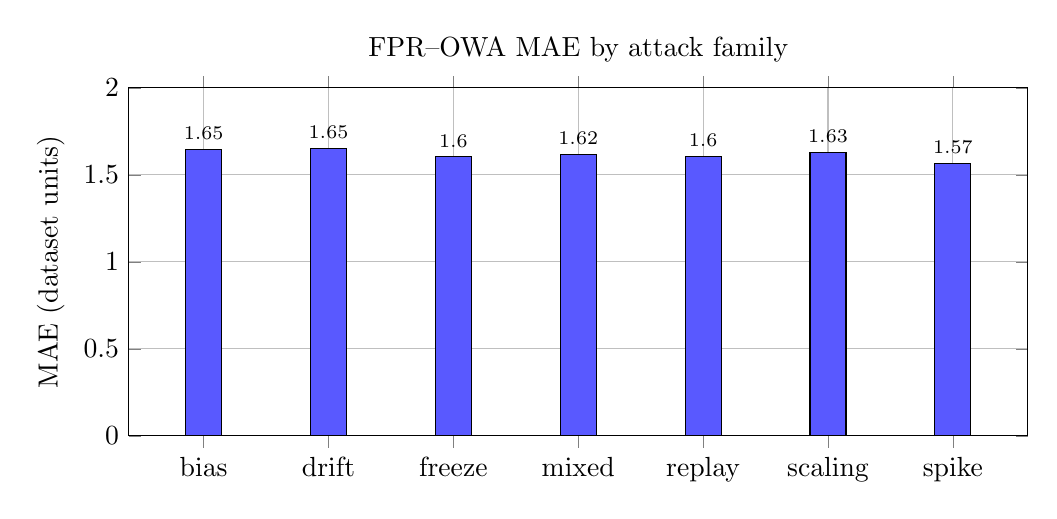
\begin{tikzpicture}
\begin{axis}[width=13cm,height=6cm,ybar,bar width=13pt,ymin=0,ymax=2.0,
 ylabel={MAE (dataset units)},symbolic x coords={bias,drift,freeze,mixed,replay,scaling,spike},
 xtick=data,nodes near coords,nodes near coords style={font=\scriptsize},
 title={FPR--OWA MAE by attack family},grid=major]
\addplot[fill=blue!65] coordinates {(bias,1.646754) (drift,1.653272) (freeze,1.603618) (mixed,1.618489) (replay,1.604410) (scaling,1.629375) (spike,1.565191)};
\end{axis}\end{tikzpicture}
\end{document}
